\documentclass{article}

\usepackage{fullpage}
\usepackage{listings}
\usepackage{graphicx}

\lstset{
  breaklines=false,
  frame=single,
  basicstyle=\footnotesize,
  keepspaces=true,
  extendedchars=true,
  escapeinside={\%*}{*)}
}

\title{From Here to Beer\\ \vspace{2 mm}{\large Android Assessment Proposal}}
\author{Ross Fenning}

\begin{document}
\maketitle

\section{Description}

The proposal is for an app for Android that suggests nearby pubs at random.
The user's current location will be used to find nearby pubs using Google
Places API and a random one within an acceptable walking distance will be
suggested. There is scope for additional features around the core proposition
such as linking to Google Maps for walking directions or allowing users
to store their favourite pubs to remind them which pubs they liked.

\section{Aims}

The target user base is that of anyone facing indecision when out looking for
pubs or who simply wishes to throw some randomness into their evening by
choosing their pub at random. Through this application, people may be suggested
pubs they otherwise would not have tried or perhaps they do not even know
those pubs existed previously.

The intention is to allow some control of the search radius to please both
people wanting immediately nearby pubs and those willing to make a longer
walk out of it. The app should also allow the ability to ``roll again'' and
choose another pub if they do not like the first suggestion.
The app should also endeavour to offer a gracefully degraded experience in
the case that services such as location or network are not available,
although its utility is likely to be very limited with those services.

The app will be developed using \emph{Behaviour-Driven Development} (BDD)
to provide
iterative and continuously tested software focused around user requirements.
Tools such as \emph{Cucumber-JVM} provide the ability to write tests based
on user stories first and then ensure each iteration does not introduce
defects to existing features. Continuous integration and the Android
Instrumentation class will allow each iteration to be tested before release.
It should also be possible to evaluate the app and its usability at each
iteration so as to use that feedback to guide the prioritisation of
further features.

\section{Specification}

The use of BDD and Cucumber-JVM means that user stories can be written to
serve the triple purpose of specification, automated testing steps and
documentation of what features are implemented so far.

The iterative
nature of any \emph{Agile} methodology means that we can adapt to change
in the requirements and features as the project develops, which teaches
us that there is limited merit in writing hundreds of requirements at the
point of project at which we have the least information -- the start. With
this in mind, this proposal will include a handful of user requirements for
an acceptable early baseline of the app and further requirements can be
shaped at the end of each iteration.

\section{User Stories}
\vspace*{\fill}
\lstinputlisting{stories/001-random-pub.feature}
\vspace*{\fill}
\lstinputlisting{stories/002-address.feature}
\vspace*{\fill}
\lstinputlisting{stories/003-directions.feature}
\vspace*{\fill}
\lstinputlisting{stories/004-change-radius.feature}
\vspace*{\fill}
\pagebreak
\vspace*{\fill}
\lstinputlisting{stories/005-another-suggestion.feature}
\vspace*{\fill}
\lstinputlisting{stories/006-favourites.feature}
\vspace*{\fill}

\section{Design}

Whilst the final design will be evolved as features are added, some mock
designs of the first activity are given in figures 1 and 2.

\vspace*{\fill}

\begin{figure}[p]
  \centering
  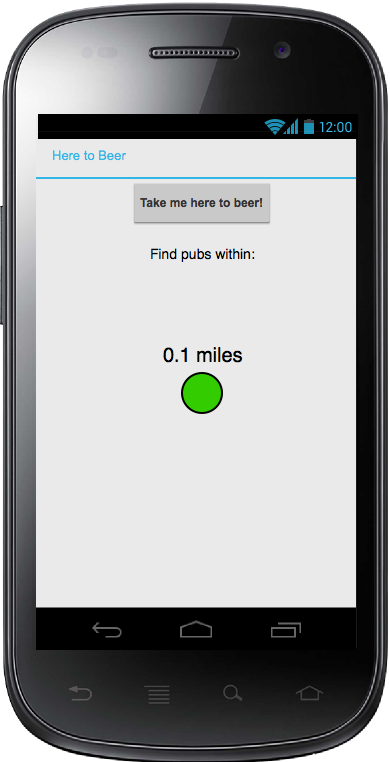
\includegraphics[height=3in]{../design/main_phone_near.png}
  \caption{User is about to request a pub within 0.1 miles}
\end{figure}
\begin{figure}[p]
  \centering
  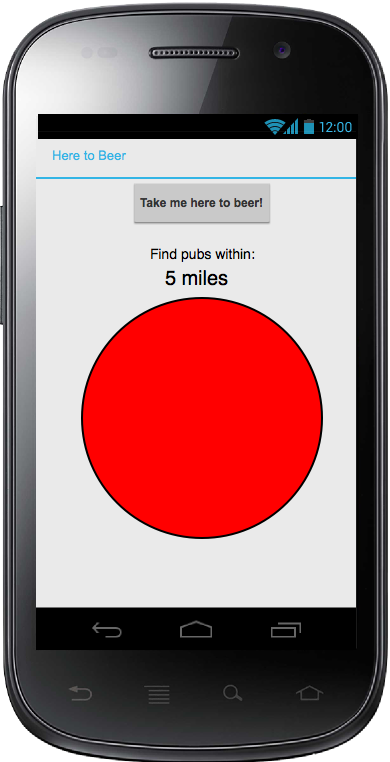
\includegraphics[height=3in]{../design/main_phone.png}
  \caption{User is about to request a pub further out up to 5 miles away}
\end{figure}

\end{document}
